\documentclass[12pt,a4paper]{scrartcl}
\usepackage[utf8]{inputenc}
\usepackage{csquotes}
\usepackage[ngerman]{babel}
\usepackage{amsmath}
\usepackage{amsfonts}
\usepackage{amssymb}
\usepackage{graphicx}
\usepackage{float}
\usepackage[backend=biber]{biblatex}
\addbibresource{./sources.bib}
\author{Leon Bentrup}
\title{NSA}
\subtitle{Globale Überwaching und Demokratie?}
\begin{document}
\maketitle
\tableofcontents
\newpage
\KOMAoptions{parskip=full}

\section{Vorwort}
Dass Geheimdienste Telefongespräche und Internetverkehr überwachen, hatte ich eigentlich nie bezweifelt. Was das wirklich bedeutet, das wurde mir aber erst vor zwei Jahren bewusst.

Als im Juni 2013 auf einmal eine ganze Ladung an Informationen über geheime Projekte des amerikanischen Geheimdienstes NSA in den Medien auftauchten, als man langsam Begriff, dass es sich dabei um etwas richtig Großes handelt, da spürte ich das ungute Gefühl, dass auch bei meinen Recherchen zu dieser GFS immer wieder auftauchte.

Es fühlt sich an, als könnte man den Schlag in die Magengrube der Freiheit spüren, den die totale Überwachung jedes Menschen der Welt darstellt.

Was im Nachhinein auch völlig logisch ist, mich aber trotzdem beunruhigt, ist die Normalität, die innerhalb der Geheimdienste herrscht. Man muss sich klar machen: Analyst, die Berufsbezeichnung für die „modernen Spione“, die die abgefangenen Daten auswerten, ist ein ganz normaler Job. Analysten wechseln Arbeitgeber und haben LinkedIn-Profile mit Lebensläufen.

Manche Dokumente zeigen Geheimdienste eher als Unternehmen, statt als geheime Organisation: Es gibt Newsletter mit „Wusstest du schon?”-Artikeln, die einen über die Geschichte des ECHELON-Programms aufklären, für das Anwenden neuer Spionage-Techniken bekommen Mitarbeiter „Skillz-Points“. In anderen Worten: Die Digitalisierung der Welt hat „Spion” zu einem Bürojob gemacht.

\section{Edward Snowden}
\begin{figure}
\centering
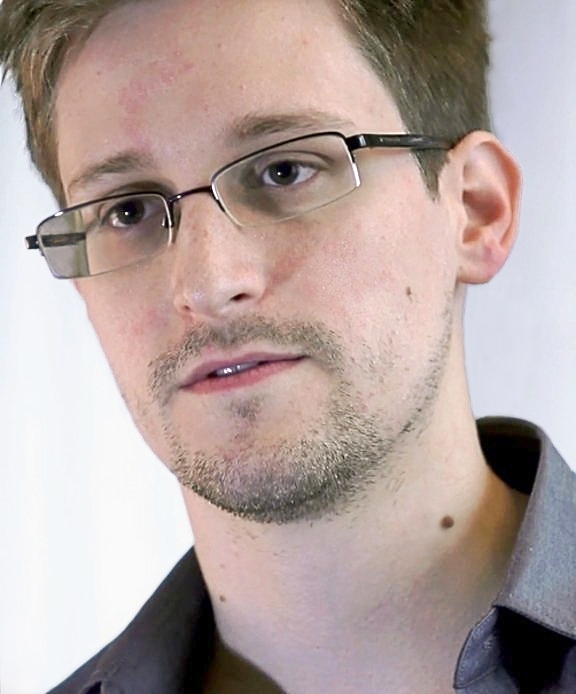
\includegraphics[width=0.4\textwidth]{images/snowden.jpg}
\caption{Edward Snowden bei seinem Interview mit Greenwald}
\end{figure}
Edward Snowden ist die zentrale Persönlichkeit der Enthüllungen. Nach langjähriger Arbeit in verschiedenen Einrichtungen der amerikanischen Regierung. Er sammelte eigenständig Millionen von Beweisen für geheime Programme der NSA und anderen Geheimdiensten, die er dann durch die Medien an die Öffentlichkeit brachte.

\subsection{Lebenslauf}
Edward Snowden wurde am 21. Juni 1983 geboren.
Da beide Eltern für die Regierung arbeiten, ist es für ihn „normal“, das gleiche zu tun.
Nach seiner Schulzeit tritt er 2004 der U.S.-Army bei, mit dem Ziel, in Irak zu kämpfen. Als er nach 3 Monaten bei der Armee einen Trainingsunfall hatte, verließ er sie wieder.
Er arbeitete danach für einige nicht-geheime Einrichtungen der Regierung, bis er 2006, beim Besuch einer Jobmesse von der CIA rekrutiert wurde, wo er unter anderem bei einem internationalen Treffen 2008 in Genf eigesetzt wurde.
\cite{wiki_snowden}

2009 wechselte er zu DELL, er kümmerte sich um die Computersysteme von Regierungskunden, darunter auch Systeme der NSA und CIA. Sein Einkommen in dieser Position betrug etwa 200~000\$ im Jahr.
Schon dort bekam er Einsicht in einige streng geheime Operationen der NSA und sammelte schon einige Dokumente als Beweiß.

Seinen entgültigen Beschluss, die Handlungen der NSA und anderer Geheimdienste an die öffentlichkeit zu bringen, fasste er 2013. In einem Interview sagte Snowden, dass der 12. März 2013 der ausschlaggebend für seine Entscheidung gewesen sei. Dort wurde der Director of National Intelligence (nationaler Geheimdienstdirektor) der USA zur Überwachung von Amerikanern befragt, und log die Mitglieder des Kongress an, obwohl er unter Eid stand.

Daraufhin gibt Snwoden seinen Job bei DELL auf und wechselte zur Dienstleistungsfirma Booz Allen Hamilton, die Personal für die NSA zur Verfügung stellte. Er war im Geheimdienst offiziell als Systemadministrator tätig, und hatte somit uneingeschränkten Zugriff auf alle Akten des Geheimdienstes. Snowden sagte, dass zu seinen Aufgaben aber auch das Überprüfen und Angreifen feindlicher Computersysteme zählte. Seine Position nannte er „Systems Analyst”

\subsection{Enthüllungen}

\begin{figure}[H]
\centering
\begin{tabular}{lr}
Australien & 15~000 Dokumente \\
Vereinigtes Köngreich & 58~000 Dokumente \\
Department of Defense & 960~000 Dokumente \\
National Security Agency & 1~700~000 Dokumente \\
& \textbf{ca. 2~700~000 Dokumente}
\end{tabular}
\caption{Zahl der von Snowden gesammelten Dokumente}
\end{figure}

Auch wenn Snowden wollte, dass die geheimen Operationen der NSA an die Öffentlichkeit geraten, war er nicht generell gegen Überwachung. Nur solle Überwachung gezielt und auf Verdacht stattfinden, und nicht so massenhaft, wie die NSA es betreibt. 

Da er also wichtige Operationen der Geheimdienste, zum Beispiel die Überwachung von bekannten Terrororganisationen, nicht gefährden wollte, musste er beim Veröffentlichen der gesammelten Dokumente vorsichtig sein. Er sichtete zunächst selbst alles und sortierte Teile aus, die nichts mit der von ihm kritisierten Massenüberwachung zu tun hatten.

Außerdem veröffentlichte er die Dokumente nicht selbst, sondern übergab sie der Filmemacherin Laura Poitras und dem Journalisten Glenn Greenwald. Sie sollten die Dokumente dann über die Medien an die Öffentlichkeit bringen.

\subsubsection{Laura Poitras}
Laura Poitras, geboren am 2. Februar 1964 in Boston, ist Produzentin und Filmemacherin. Sie arbeitet seit 2005 an einer Filmreihe über die Welt nach dem 11. September 2001. Nachdem sie den ersten Film der Trilogie veröffentlicht hat, wird sie regelmäßig an der amerikanischen Grenze kontrolliert und befragt. Aus diesem Grund zieht sie nach Berlin um, als sie mit ihrem Film „Citizenfour” beginnt. Sie befürchtet, dass ihr Filmmaterial beschlagnahmt wird.\cite{praxisfilms}

\subsubsection{Glenn Greenwald}
Der amerikanische Journalist Glenn Greenwald, der am 6. März 1967 in New York geboren wurde, ist die zweite Person, die Snowden kontaktierte. Er studierte Philosophie und Rechtswissenschaften.\cite{wiki_greenwald} Von 1996 bis 2005 arbeitete er in einer eigenen Anwaltskanzlei, die sich auf Verfassungs- und Bürgerrechte (von US-Bürgern) spezialisierte.\cite{unclaimed_response}

In seinen Blog „Unclaimed Territory“ schrieb Greenwald bis 2007 unter anderem über frühere Affären der NSA, bis er später zum Online-Magazin „salon.com“ und schließlich im Juni 2012 zur britischen Tageszeitung „The Guardian” wechselte. Im Guardian veröffentlichte Greenwald auch den ersten Artikel über das Snowden-Material.\cite{wiki_greenwald}

2014 gründete er zusammen mit Laura Poitras die Nachrichtenseite „The Intercept“.\cite{intercept_about}

\section{Überwachung}
% Allgemeines

\subsection{XKeyscore}


\subsection{Five Eyes}

\subsection{TEMPORA}

\section{Verhältnis zu Deutschland}

\subsection{Partnerschaft mit der NSA}

\subsection{Operation Eikonal}

\section{Geheimdienste in Deutschland}

\subsection{MAD}

\subsection{BfV}

\subsection{BND}

\section{Fazit}

\newpage
\printbibliography

\end{document}
